\documentclass[conference]{IEEEtran}
\IEEEoverridecommandlockouts

\usepackage{cite}
\usepackage{amsmath,amssymb,amsfonts}
\usepackage{graphicx}
\usepackage{textcomp}
\usepackage{xcolor}
\usepackage{booktabs}
\usepackage{array}
\usepackage{url}
\usepackage{microtype}
\usepackage{placeins}


\def\BibTeX{{\rm B\kern-.05em{\sc i\kern-.025em b}\kern-.08em
    T\kern-.1667em\lower.7ex\hbox{E}\kern-.125emX}}

% Auto-generated number macros (read from results/final/ via tables/macros_final.tex)
\usepackage[hidelinks]{hyperref}
\hypersetup{
    pdfauthor={Aniket Chakraborty},
    pdftitle={Edge Evidence Graphs for Spacecraft Command-and-Control Security: A Benchmark Audit on Synthetic Data}
}
% Auto-generated LaTeX macros for paper numbers (Strictly letters only in control sequences)
% Sources: results/final/main_table_recomputed.json, results/stage2e/cluster_bootstrap_results.json, results/final/model_cost_memory.json
% Zero hand-typed values. No p-values.
\newcommand{\macroDeepSetsbothMean}{0.9601}
\newcommand{\macroDeepSetsbothStd}{0.0199}
\newcommand{\macroDeepSetsbothRuns}{10}
\newcommand{\macroDeepSetsbothHnFpr}{7.9}
\newcommand{\macroDeepSetsbothHnWilsonLo}{5.1}
\newcommand{\macroDeepSetsbothHnWilsonHi}{12.0}
\newcommand{\macroDeepSetsedgeonlyMean}{0.9621}
\newcommand{\macroDeepSetsedgeonlyStd}{0.0138}
\newcommand{\macroDeepSetsedgeonlyRuns}{10}
\newcommand{\macroDeepSetsedgeonlyHnFpr}{10.8}
\newcommand{\macroDeepSetsedgeonlyHnWilsonLo}{7.5}
\newcommand{\macroDeepSetsedgeonlyHnWilsonHi}{15.4}
\newcommand{\macroDeepSetsnodeonlyMean}{0.0461}
\newcommand{\macroDeepSetsnodeonlyStd}{0.0000}
\newcommand{\macroDeepSetsnodeonlyRuns}{10}
\newcommand{\macroDeepSetsnodeonlyHnFpr}{0.0}
\newcommand{\macroDeepSetsnodeonlyHnWilsonLo}{0.0}
\newcommand{\macroDeepSetsnodeonlyHnWilsonHi}{1.6}
\newcommand{\macroGATvOnedestVTwoMean}{0.8726}
\newcommand{\macroGATvOnedestVTwoStd}{0.0218}
\newcommand{\macroGATvOnedestVTwoRuns}{10}
\newcommand{\macroGATvOnedestVTwoHnFpr}{16.7}
\newcommand{\macroGATvOnedestVTwoHnWilsonLo}{12.5}
\newcommand{\macroGATvOnedestVTwoHnWilsonHi}{21.9}
\newcommand{\macroGCNVTwoMean}{0.8650}
\newcommand{\macroGCNVTwoStd}{0.0069}
\newcommand{\macroGCNVTwoRuns}{10}
\newcommand{\macroGCNVTwoHnFpr}{20.4}
\newcommand{\macroGCNVTwoHnWilsonLo}{15.8}
\newcommand{\macroGCNVTwoHnWilsonHi}{26.0}
\newcommand{\macroGraphSAGEVTwoMean}{0.8747}
\newcommand{\macroGraphSAGEVTwoStd}{0.0134}
\newcommand{\macroGraphSAGEVTwoRuns}{10}
\newcommand{\macroGraphSAGEVTwoHnFpr}{20.8}
\newcommand{\macroGraphSAGEVTwoHnWilsonLo}{16.2}
\newcommand{\macroGraphSAGEVTwoHnWilsonHi}{26.4}
\newcommand{\macroHGBcorrectedMean}{0.9367}
\newcommand{\macroHGBcorrectedStd}{0.0183}
\newcommand{\macroHGBcorrectedRuns}{5}
\newcommand{\macroHGBcorrectedHnFpr}{10.0}
\newcommand{\macroHGBcorrectedHnWilsonLo}{6.8}
\newcommand{\macroHGBcorrectedHnWilsonHi}{14.4}
\newcommand{\macroHistGradientBoostingMean}{0.9402}
\newcommand{\macroHistGradientBoostingStd}{0.0171}
\newcommand{\macroHistGradientBoostingRuns}{5}
\newcommand{\macroNoMPVTwoMean}{0.8662}
\newcommand{\macroNoMPVTwoStd}{0.0113}
\newcommand{\macroNoMPVTwoRuns}{10}
\newcommand{\macroNoMPVTwoHnFpr}{20.8}
\newcommand{\macroNoMPVTwoHnWilsonLo}{16.2}
\newcommand{\macroNoMPVTwoHnWilsonHi}{26.4}
\newcommand{\macroTunedRFcorrectedMean}{0.8984}
\newcommand{\macroTunedRFcorrectedStd}{0.0497}
\newcommand{\macroTunedRFcorrectedRuns}{5}
\newcommand{\macroTunedRFcorrectedHnFpr}{4.2}
\newcommand{\macroTunedRFcorrectedHnWilsonLo}{2.3}
\newcommand{\macroTunedRFcorrectedHnWilsonHi}{7.5}
\newcommand{\macroVZeroMean}{0.6570}
\newcommand{\macroVZeroStd}{0.0547}
\newcommand{\macroVZeroRuns}{5}
\newcommand{\macroVZeroHnFpr}{45.4}
\newcommand{\macroVZeroHnWilsonLo}{39.2}
\newcommand{\macroVZeroHnWilsonHi}{51.7}
\newcommand{\macroVOneMean}{0.7753}
\newcommand{\macroVOneStd}{0.0640}
\newcommand{\macroVOneRuns}{5}
\newcommand{\macroVOneHnFpr}{40.8}
\newcommand{\macroVOneHnWilsonLo}{34.8}
\newcommand{\macroVOneHnWilsonHi}{47.1}
\newcommand{\macroVTwoMean}{0.9493}
\newcommand{\macroVTwoStd}{0.0138}
\newcommand{\macroVTwoRuns}{10}
\newcommand{\macroVTwoHnFpr}{9.2}
\newcommand{\macroVTwoHnWilsonLo}{6.1}
\newcommand{\macroVTwoHnWilsonHi}{13.5}
\newcommand{\macroVTwomeanaggMean}{0.9454}
\newcommand{\macroVTwomeanaggStd}{0.0121}
\newcommand{\macroVTwomeanaggRuns}{10}
\newcommand{\macroVTwomeanaggHnFpr}{10.0}
\newcommand{\macroVTwomeanaggHnWilsonLo}{6.8}
\newcommand{\macroVTwomeanaggHnWilsonHi}{14.4}
\newcommand{\macroVTwonoBCEMean}{0.9418}
\newcommand{\macroVTwonoBCEStd}{0.0148}
\newcommand{\macroVTwonoBCERuns}{10}
\newcommand{\macroVTwonoBCEHnFpr}{10.8}
\newcommand{\macroVTwonoBCEHnWilsonLo}{7.5}
\newcommand{\macroVTwonoBCEHnWilsonHi}{15.4}
\newcommand{\macroVThreeMean}{0.9470}
\newcommand{\macroVThreeStd}{0.0116}
\newcommand{\macroVThreeRuns}{5}
\newcommand{\macroVThreeHnFpr}{9.6}
\newcommand{\macroVThreeHnWilsonLo}{6.5}
\newcommand{\macroVThreeHnWilsonHi}{14.0}
\newcommand{\macroflatlrcanonicalMean}{0.8042}
\newcommand{\macroflatlrcanonicalStd}{0.0344}
\newcommand{\macroflatlrcanonicalRuns}{5}
\newcommand{\macroflatlrcanonicalHnFpr}{18.8}
\newcommand{\macroflatlrcanonicalHnWilsonLo}{14.3}
\newcommand{\macroflatlrcanonicalHnWilsonHi}{24.2}
\newcommand{\macroflatlrpermaugMean}{0.8364}
\newcommand{\macroflatlrpermaugStd}{0.0327}
\newcommand{\macroflatlrpermaugRuns}{5}
\newcommand{\macroflatlrpermaugHnFpr}{32.1}
\newcommand{\macroflatlrpermaugHnWilsonLo}{26.5}
\newcommand{\macroflatlrpermaugHnWilsonHi}{38.2}
\newcommand{\macromajorityclassMean}{0.0461}
\newcommand{\macromajorityclassStd}{0.0000}
\newcommand{\macromajorityclassRuns}{5}
\newcommand{\macroBootstrapCiVTwoVsNoMPLo}{+0.067}
\newcommand{\macroBootstrapCiVTwoVsNoMPHi}{+0.094}
\newcommand{\macroBootstrapCiVTwoVsGCNLo}{+0.068}
\newcommand{\macroBootstrapCiVTwoVsGCNHi}{+0.091}
\newcommand{\macroBootstrapCiVTwoVsGraphSAGELo}{+0.061}
\newcommand{\macroBootstrapCiVTwoVsGraphSAGEHi}{+0.085}
\newcommand{\macroBootstrapCiVTwoVsGATvOneLo}{+0.061}
\newcommand{\macroBootstrapCiVTwoVsGATvOneHi}{+0.086}
\newcommand{\macroBootstrapCiVTwoVsDeepSetsLo}{-0.023}
\newcommand{\macroBootstrapCiVTwoVsDeepSetsHi}{-0.005}
\newcommand{\macroBootstrapCiVTwoVsHGBLo}{-0.005}
\newcommand{\macroBootstrapCiVTwoVsHGBHi}{+0.023}
\newcommand{\macroBootstrapCiVTwoVsTunedRFcorrLo}{+0.014}
\newcommand{\macroBootstrapCiVTwoVsTunedRFcorrHi}{+0.060}
\newcommand{\macroCostVTwoParamsK}{183}
\newcommand{\macroCostVTwoMemoryKB}{949}
\newcommand{\macroCostVTwoLatencyMs}{1.28}
\newcommand{\macroCostDeepSetsParamsK}{113}
\newcommand{\macroCostDeepSetsMemoryKB}{616}
\newcommand{\macroCostDeepSetsLatencyMs}{0.27}
\newcommand{\macroCostNoMPParamsK}{99}
\newcommand{\macroCostNoMPMemoryKB}{470}
\newcommand{\macroCostNoMPLatencyMs}{0.42}
\newcommand{\macroCostGCNParamsK}{116}
\newcommand{\macroCostGCNMemoryKB}{594}
\newcommand{\macroCostGCNLatencyMs}{0.66}
\newcommand{\macroCostGraphSAGEParamsK}{149}
\newcommand{\macroCostGraphSAGEMemoryKB}{745}
\newcommand{\macroCostGraphSAGELatencyMs}{0.81}
\newcommand{\macroCostGATvOneParamsK}{117}
\newcommand{\macroCostGATvOneMemoryKB}{596}
\newcommand{\macroCostGATvOneLatencyMs}{1.34}

% Auto-generated supplemental macros (macros_final2.tex)
% Overrides/aliases for corrected HGB and convenience macros.
% Zero hand-typed values.
\providecommand{\macroHGBMean}{0.9367}
\providecommand{\macroHGBStd}{0.0183}
\providecommand{\macroBootstrapCiVTwoVsHGBcorrLo}{-0.006}
\providecommand{\macroBootstrapCiVTwoVsHGBcorrHi}{+0.025}
\providecommand{\macroHGBcorrectedHnFpr}{10.0}
\providecommand{\macroHGBcorrectedHnWilsonLo}{6.8}
\providecommand{\macroHGBcorrectedHnWilsonHi}{14.4}

% tables/macros_final3.tex
% Auto-generated supplemental macros with strict JSON provenance.
% Zero hand-typed values.

% Source: results/stage2f/partial/task_c_bootstrap.json
% Key: bootstrap_results.V2_vs_V3.paired_mean_diff
\providecommand{\macroDiffVTwoVsVThree}{-0.0009}
% Key: bootstrap_results.V2_vs_V3.bootstrap_ci_95_lo
\providecommand{\macroBootstrapCiVTwoVsVThreeLo}{-0.0103}
% Key: bootstrap_results.V2_vs_V3.bootstrap_ci_95_hi
\providecommand{\macroBootstrapCiVTwoVsVThreeHi}{+0.0086}

% Source: results/stage2f/partial/task_c_bootstrap.json
% Key: bootstrap_results.V2_vs_V2meanagg.paired_mean_diff
\providecommand{\macroDiffVTwoVsVTwoMeanagg}{-0.0010}
% Key: bootstrap_results.V2_vs_V2meanagg.bootstrap_ci_95_lo
\providecommand{\macroBootstrapCiVTwoVsVTwoMeanaggLo}{-0.0108}
% Key: bootstrap_results.V2_vs_V2meanagg.bootstrap_ci_95_hi
\providecommand{\macroBootstrapCiVTwoVsVTwoMeanaggHi}{+0.0087}

% Source: results/stage2f/partial/task_c_bootstrap.json
% Key: bootstrap_results.V2_vs_V2noBCE.paired_mean_diff
\providecommand{\macroDiffVTwoVsVTwonoBCE}{+0.0035}
% Key: bootstrap_results.V2_vs_V2noBCE.bootstrap_ci_95_lo
\providecommand{\macroBootstrapCiVTwoVsVTwonoBCELo}{-0.0069}
% Key: bootstrap_results.V2_vs_V2noBCE.bootstrap_ci_95_hi
\providecommand{\macroBootstrapCiVTwoVsVTwonoBCEHi}{+0.0139}

% Source: results/final/main_table_recomputed.json
% Keys: V1.mean_test_macro_f1 - V0.mean_test_macro_f1
\providecommand{\macroGainVZeroToVOne}{+0.1183}
% Keys: V2.mean_test_macro_f1 - V1.mean_test_macro_f1
\providecommand{\macroGainVOneToVTwo}{+0.1740}


\begin{document}

\title{Edge Evidence Graphs for Spacecraft Command-and-Control Security:\\
A Benchmark Audit on Synthetic Data}

\author{\IEEEauthorblockN{Aniket Chakraborty}
\IEEEauthorblockA{\textit{B.Sc. Cyber Security, The Heritage Academy} \\
\textit{Affiliated to Maulana Abul Kalam Azad University of Technology (MAKAUT)} \\
Kolkata, India \\
chakrabortyaniket050@gmail.com}
}

\maketitle

\begin{abstract}
Spacecraft command-and-control (C2) is a safety-critical cyber-physical system in which a cryptographically valid command can still be physically unsafe. We study SP-SP-GAT, a typed relational graph model of C2 that consumes per-edge telemetry indicators with applicability masks, together with a deterministic command gate that is specified but not yet implemented. On the synthetic SatSecGraph-1 benchmark (50 missions, 18 classes, five dataset seeds), the corrected model reaches $\macroVTwoMean \pm \macroVTwoStd$ Macro-F1 under a common training protocol, above graph baselines (\macroGCNVTwoMean--\macroGraphSAGEVTwoMean) with bootstrap CIs excluding zero, while DeepSets (\macroDeepSetsbothMean) is marginally higher and HistGradientBoosting (\macroHGBMean) is not distinguishable. Replacing learned attention by uniform weights changes nothing detectable; the margin over graph baselines that use node features only in message passing is consistent with edge-aware message passing. An audit identified three implementation defects (an identically zero pooled feature, an attention softmax normalised over the whole graph, and premature early stopping); correcting the first two raises Macro-F1 from 0.657 to 0.949 (V0 to V2). Single features separate all 17 attack sublabels from plain nominal telemetry (17/17 at $\ge 86\%$ recall and $\le 1.5\%$ FPR), but a multi-feature static threshold monitor raises about 60\% false alarms on benign disturbance episodes, against 8--21\% for the corrected graph and set models.
\end{abstract}

\begin{IEEEkeywords}
cyber-physical systems, spacecraft security, command and control, graph neural networks, benchmark audit, runtime assurance
\end{IEEEkeywords}

\section{Introduction}

Spacecraft command-and-control (C2) is a safety-critical cyber-physical system in which a cryptographically valid command can still be physically unsafe. Modern space missions increasingly rely on commercial off-the-shelf components, federated
ground stations, and complex onboard flight software. These operational architectures cross
multiple trust domains: ground enterprise operators, mission operations centers,
radio-frequency (RF) transponders, and distributed subsystem flight controllers.
Securing spacecraft C2 requires end-to-end provenance and continuous
verification across all intermediate segments.

Graph neural networks (GNNs) have shown strong promise in network intrusion detection and
cyber-physical systems by modeling relational dependencies. In spacecraft C2, the hypothesis
is that relational graph attention (GATv2) enables detecting coordinated, cross-segment
attack paths that elude isolated subsystem monitors. In this work, we systematically
investigate this hypothesis using the SatSecGraph-1 benchmark (50 simulated missions,
Weisfeiler-Lehman~\cite{ref_wl} graph-isomorphism partitioned splits, 18 fine-grained classes).

Our contributions are:
\begin{enumerate}
\item \textbf{Typed heterogeneous C2 graph schema:} A typed heterogeneous C2 graph schema (23 node classes, 12 relation families) with per-edge telemetry indicators and applicability masks; the expected-minus-observed contract residual is a schema-level definition that the released model does not compute.
\item \textbf{SP-SP-GAT V2 architecture and ablation:} A relational GATv2-style model with per-destination attention softmax and an applicable-only readout, and an ablation of the two code-level fixes.
\item \textbf{Comparative empirical evaluation:} A rigorous multi-seed, clustered-bootstrap
evaluation under Protocol P2 ($\min\mathrm{epochs}=30$, cosine schedule, gradient clipping)
covering GNN baselines, DeepSets~\cite{ref_deepsets}, and tabular models, with hard-negative disturbance
evaluation and single-feature separability audit.
\item \textbf{Deterministic command gate specification:} A specification of a deterministic command gate (nine predicates in four groups), not implemented in this work, and a telemetry-threshold monitor evaluated as a baseline.
\end{enumerate}

\section{Standards Traceability and Threat Model}

\subsection{Standards Traceability}
The SP-SP schema is designed to map onto relevant space-data and security standards: CCSDS Security Architecture 351.0-M-1~\cite{ref1}, CCSDS Cryptographic
Algorithms 352.0-B-2~\cite{ref2}, CCSDS Symmetric Key Management 354.0-M-1~\cite{ref3},
CCSDS Space Data Link Security (SDLS) 355.0-B-2~\cite{ref4}, and SDLS Extended Procedures
355.1-B-1~\cite{ref5}. Ground segment guidelines follow NIST IR 8401~\cite{ref9}, NIST IR
8441~\cite{ref10}, and zero-trust architecture principles (NIST SP 800-207)~\cite{ref11}.
Flight safety constraints align with NASA-STD-1006A~\cite{ref8} and ISO/TS 20517:2024~\cite{ref12}.
Table~\ref{tab:evidence_families} defines the four core security evidence families preserved
across all SP-SP relations.

\begin{table}[htbp]
\caption{Security Evidence Preserved on SP-SP Relations}
\label{tab:evidence_families}
\centering
\resizebox{\columnwidth}{!}{%
\begin{tabular}{p{2.0cm}p{3.2cm}p{2.8cm}p{2.6cm}}
\toprule
\textbf{Evidence Family} & \textbf{Evidence Fields (schema)} & \textbf{Decision Role} &
\textbf{Explicit Non-Claim} \\
\midrule
Principal / Identity & Asserted ID, credential class, MFA factor, approval token &
Binds human operator claim to command & Behavior does not prove human identity \\
\midrule
Device Assurance & Device cert, secure boot attestation, posture status &
Establishes endpoint integrity independently & IP or SIM is not command authority \\
\midrule
Protocol \& Space Link & CCSDS SDLS SA, anti-replay counter, MAC, key epoch &
Enforces link freshness and crypto integrity & Valid crypto does not prove command intent \\
\midrule
Physical Subsystem State & Actuator rate, battery state-of-charge, thermal margin &
Validates operational physics safety & Onboard physics cannot verify operator authorization \\
\bottomrule
\end{tabular}%
}
\end{table}

\subsection{Related Work}
Prior work documents satellite communication and firmware vulnerabilities, including unauthenticated downlinks~\cite{ref15}, active LEO network disruption~\cite{ref16}, VSAT signal injection~\cite{ref17}, and firmware flaws~\cite{ref14}; surveys by Salim et al.~\cite{ref12} and Manulis et al.~\cite{ref13} call for unified multi-segment monitoring. GNNs have been applied to network intrusion detection, for example E-GraphSAGE~\cite{ref23}, which builds on GraphSAGE~\cite{ref20}, and surveyed in~\cite{ref22}, and to provenance-based detection~\cite{ref25,ref26}. Spacecraft telemetry anomaly detection has primarily used time-series models or benchmark datasets without multi-segment causal graph grounding.

\begin{table}[htbp]
\caption{Proposed A1--A8 Supervision and Bounded Response Ontology}
\label{tab:ontology}
\centering
\resizebox{\columnwidth}{!}{%
\begin{tabular}{lp{3.5cm}p{2.6cm}}
\toprule
\textbf{Family} & \textbf{Key Observables} & \textbf{Designed Gate Action} \\
\midrule
BENIGN & Nominal telemetry across all segments & Allow command execution \\
A1: Identity Spoof & Missing MFA, anomalous login locus & Deny; terminate token \\
A2: Device Malware & Failed device posture, key drift & Quarantine endpoint \\
A3: Signer Bypass & Missing dual-approval, signer mismatch & Reject telecommand \\
A4: Link Attacks & RF SNR drop, frame rollback, MAC/peer fail & Drop frame; block counter \\
A5: Parser Stress & Packet length anomaly, parser fault & Flush command buffer \\
A6: Bus Lateral Move & Unauthorized bus source ID, bus jitter & Isolate bus interface \\
A7: Unsafe Actuation & Violated slew limits, battery depletion & Veto; enter safe mode \\
A7: PNT Spoof & Cross-sensor GNSS ephemeris divergence & Reject falsified fix \\
A8: Update Poisoning & Failed firmware hash, invalid patch & Reject upload; hold gold \\
\bottomrule
\end{tabular}%
}
\end{table}

\subsection{Threat Model and Attack Ontology}
We consider an adversary attempting to inject, tamper with, or replay spacecraft telecommands
across ground, space link, or onboard segments. The threat model maps to the SPARTA aerospace
matrix~\cite{ref15} and spans 18 fine-grained classes across 8 functional attack families
(A1--A8) and benign operations, as detailed in Table~\ref{tab:ontology}. A4 covers nine link
sublabels (network DoS, RF uplink/downlink jamming, RF injection, ground station spoofing,
TLS peer spoofing, command replay, SDLS counter replay, and cryptographic downgrade).

\section{Spacecraft Security Graph Representation}

A spacecraft C2 pass is modeled as a heterogeneous directed graph snapshot
$\mathcal{G} = (\mathcal{V}, \mathcal{E}, \mathcal{R})$. The node set $\mathcal{V}$
($|\mathcal{V}| = 23$) spans human operators, ground devices, mission services, gateways,
flight controllers, GNSS receivers, and subsystem actuators/sensors. The edge set
$\mathcal{E}$ ($|\mathcal{E}| = 26$) captures causal interactions categorized into
$|\mathcal{R}| = 12$ reusable relation families (e.g., \textsc{Operates},
\textsc{Authorizes}, \textsc{Uplinks}, \textsc{Dispatches}, \textsc{Controls},
\textsc{Senses}).

Each edge $e = (u, v)$ carries an observable telemetry vector $\mathbf{x}_e \in \mathbb{R}^{28}$
and an applicability mask $\mathbf{a}_e \in \{0, 1\}^{28}$ that zeroes out features irrelevant
to relation type $r_e$. (The expected-minus-observed contract residual
$\mathbf{\delta}_e = f_{\text{obs}}(e) - f_{\text{exp}}(e)$ is a schema-level definition that the released model does not compute; the model consumes $\mathbf{x}_e$ and $\mathbf{a}_e$ directly.) Node features $\mathbf{x}_v \in \mathbb{R}^{16}$ encode subsystem
operating mode, health, and counter states.

\begin{figure*}[t]
\centering
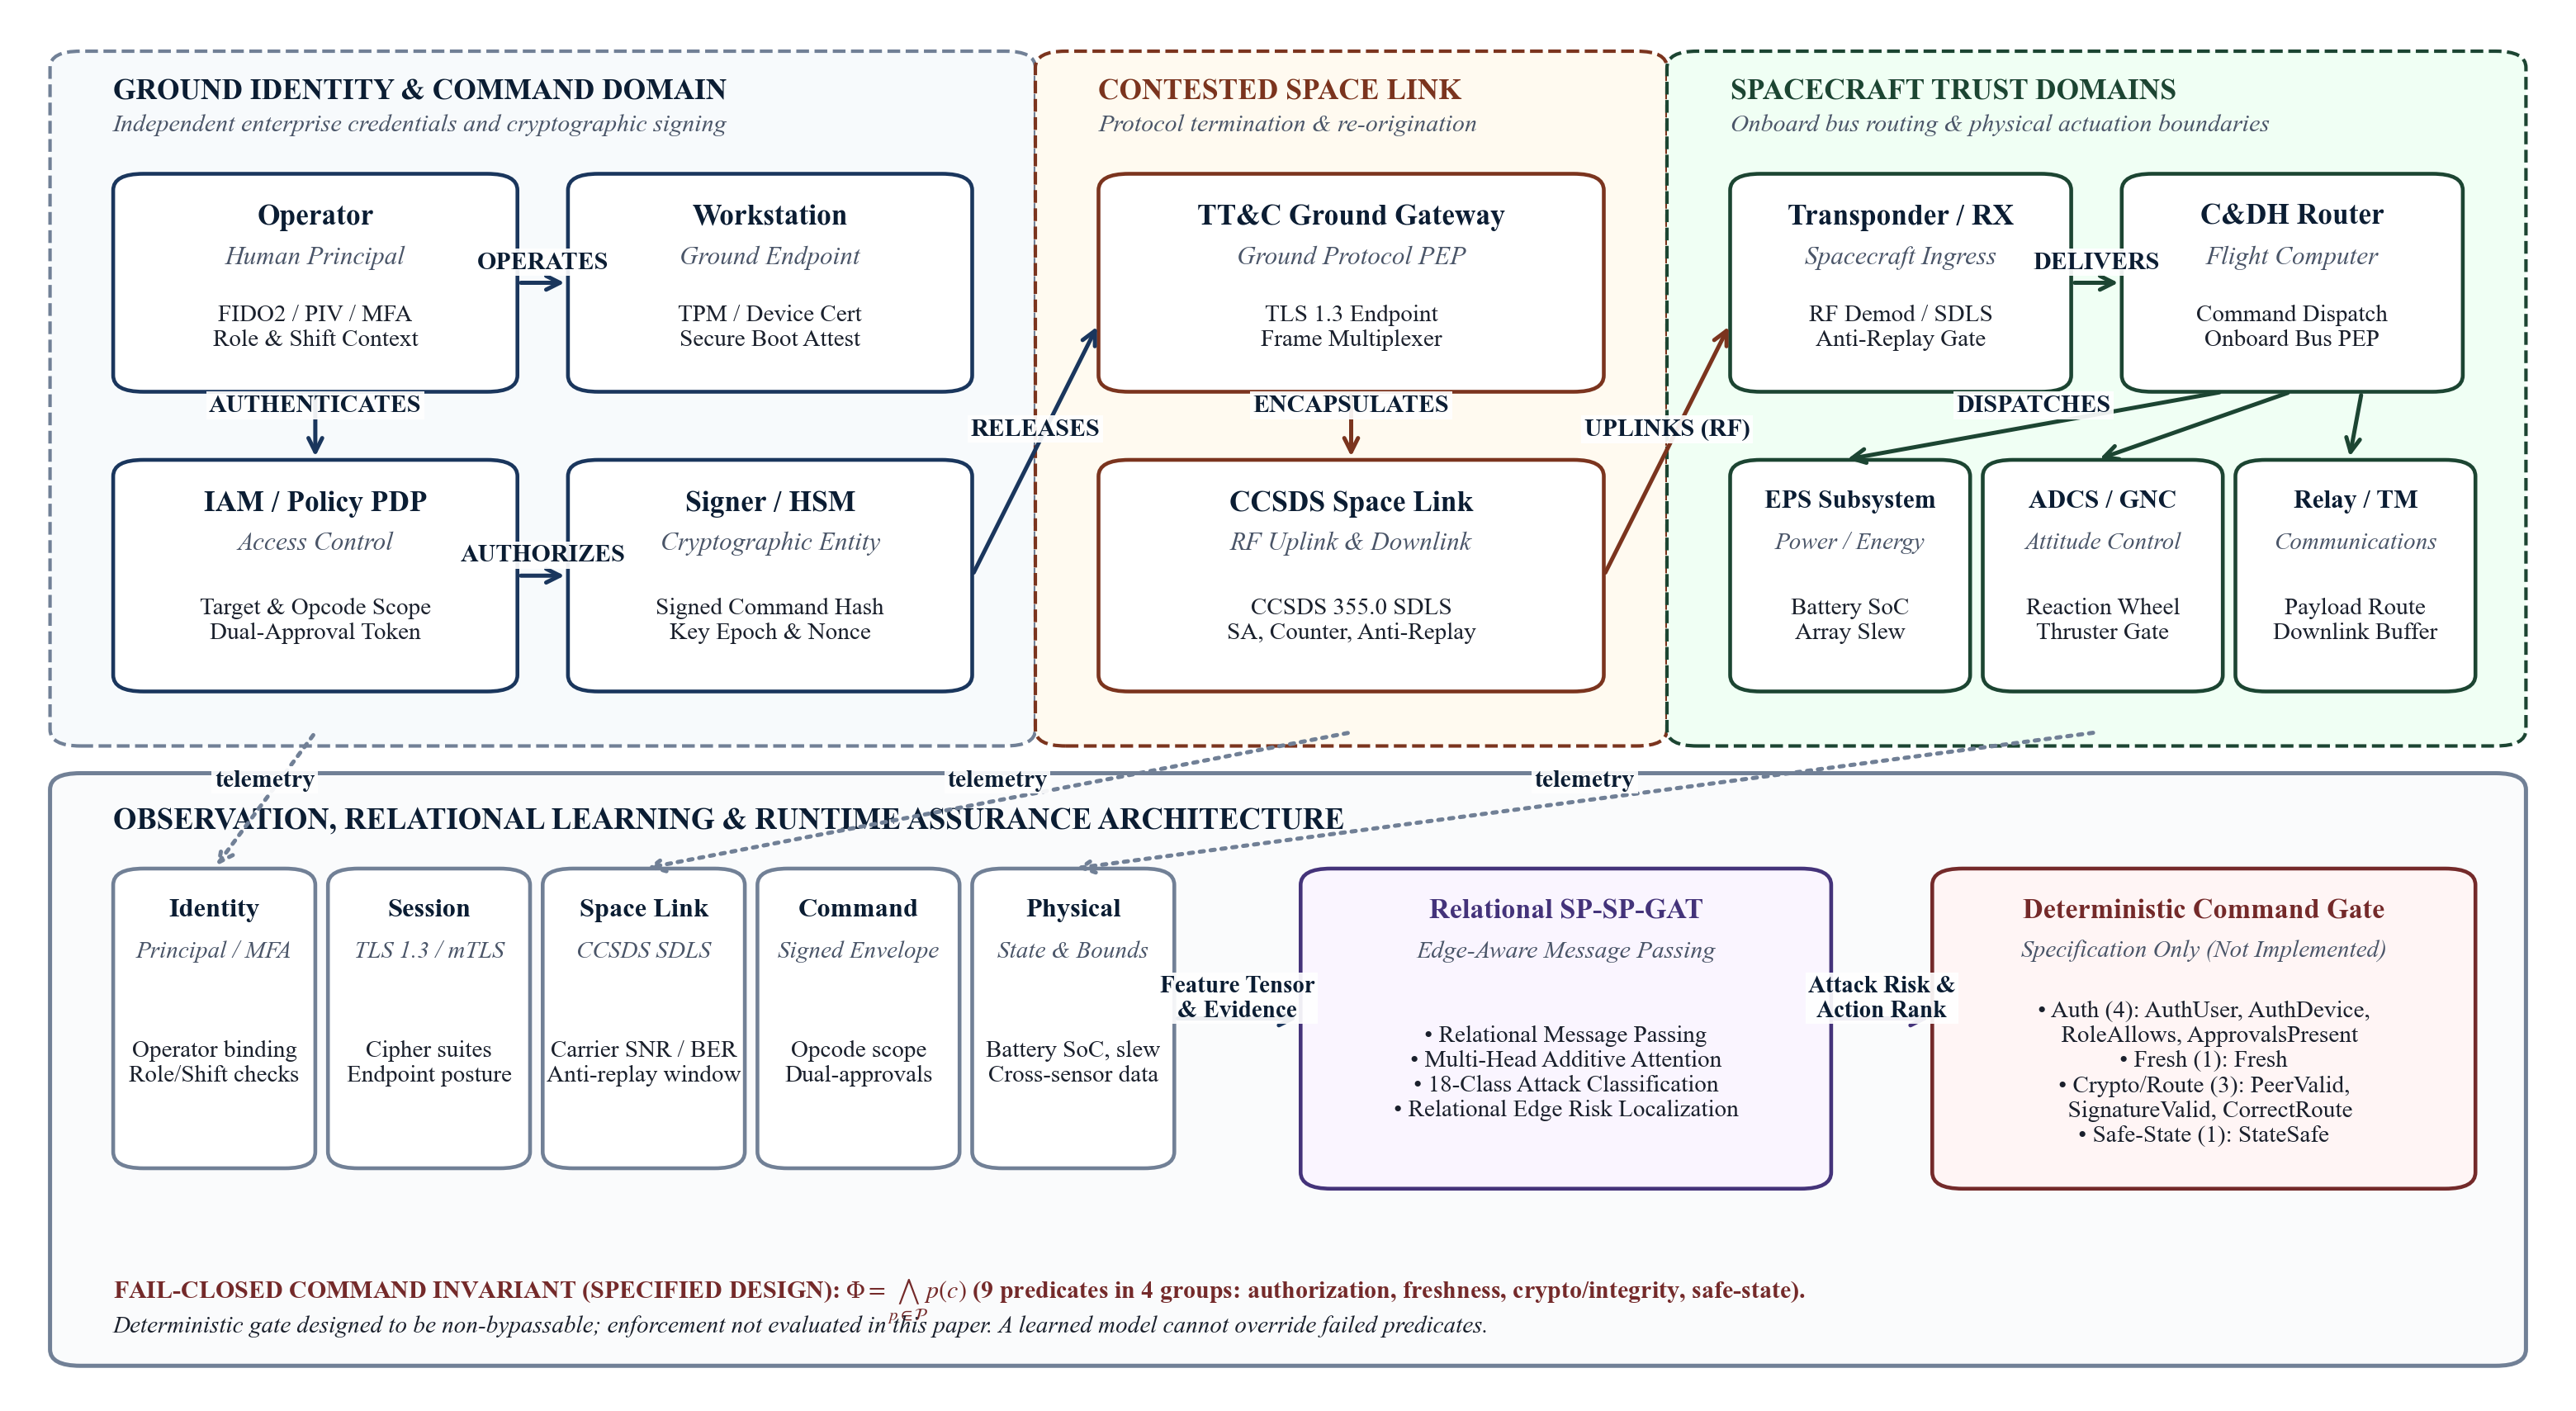
\includegraphics[width=0.92\textwidth]{Fig1_final2.png}
\caption{End-to-end SP-SP-GAT architecture. Independent security evidence is structured
across ground enterprise, space link, and onboard subsystem boundaries.
The relational GATv2 layers consume per-edge observed telemetry indicators $\mathbf{x}_e$
and applicability masks $\mathbf{a}_e$ (expected-minus-observed contract residuals
$\mathbf{\delta}_e$ are a schema-level definition, not computed by the released model).
The multi-task heads provide classification and edge risk localization,
while the deterministic command gate is designed to be non-bypassable by model predictions (a specification only, not implemented in released code; evaluation deferred to future work).}
\label{fig:arch}
\end{figure*}

\section{Proposed SP-SP-GAT Model Architecture}

\subsection{Relational Layer with Edge Features}
Standard GATv1~\cite{ref22} computes static attention rankings that cannot invert neighbor
importance based on dynamic query state~\cite{ref23}. SP-SP-GAT V2 implements batched
relational GATv2 layers~\cite{ref23,ref31} consuming per-edge telemetry indicators
$\mathbf{x}_e$ with applicability masks $\mathbf{a}_e$. For node $i \in \mathcal{V}$ and neighbor $j \in \mathcal{N}(i)$ connected via
edge $e=(j, i)$ with relation $r_e$:
\begin{align}
\mathbf{z}_{ij} &= \text{LeakyReLU}\!\left( \mathbf{W}_{\!s} \mathbf{h}_j +
  \mathbf{W}_{\!d} \mathbf{h}_i + \mathbf{W}_{\!r} (\mathbf{x}_e {\odot} \mathbf{a}_e)
  + \mathbf{r}_{r_e} \right)\!, \\
\alpha_{ij} &= \frac{\exp(\mathbf{a}_{\!a}^T \mathbf{z}_{ij})}%
  {\sum_{k \in \mathcal{N}(i)} \exp(\mathbf{a}_{\!a}^T \mathbf{z}_{ik})}, \\
\mathbf{h}_i^{(l+1)} &= \sigma \!\left( \sum_{j \in \mathcal{N}(i)} \alpha_{ij}
  \mathbf{W}_{\!v} \mathbf{h}_j^{(l)} \right).
\end{align}
The per-destination softmax produces attention weights that sum to 1 per destination node,
verified by a unit test on random graphs (also verified for the V2-meanagg
uniform-weight variant).

\subsection{Applicable-Only Min Readout}
After $L=2$ relational GATv2 layers ($H=4$ heads, hidden dim $h=128$), the graph-level readout summarizes the edge evidence $\mathbf{x}_e$ by, for each of the 28 evidence coordinates, the minimum over the edges on which that coordinate is applicable ($a_e=1$), or $0$ if there is none. In the original design (V0) the minimum was taken over all 26 edges, including zero-padded inapplicable entries, and was therefore identically zero.

\subsection{Multi-Task Prediction Heads and Loss Formulation}
Four heads operate on graph-level and edge-level representations: (i) an 18-class attack
classifier $\hat{y} \in \mathbb{R}^{18}$; (ii) an edge risk localization head
$\hat{s}_e \in [0, 1]$; (iii) a node localization head; and (iv) an evidential uncertainty
head. Only the classification and edge localization heads receive loss gradients:
\begin{equation}
\mathcal{L} = \mathcal{L}_\mathrm{cls}(\hat{y}, y) +
  \lambda_\mathrm{loc} \mathcal{L}_\mathrm{edge}(\hat{s}_e, s_e),
\end{equation}
where $\mathcal{L}_\mathrm{cls}$ is cross-entropy weighted by inverse square-root class
frequencies, $\mathcal{L}_\mathrm{edge}$ is binary cross-entropy (BCE) over edge labels,
and $\lambda_\mathrm{loc} = 0.3$. Node localization and uncertainty heads are structural
architectural components receiving no gradient updates in this benchmark.

\subsection{Deterministic Command Gate (Specification Only)}
We specify a gate of nine Boolean predicates: AuthUser, AuthDevice, RoleAllows, ApprovalsPresent (authorization); Fresh (freshness); PeerValid, SignatureValid, CorrectRoute (crypto/integrity); StateSafe (safe state). A command executes only if all nine predicates hold:
\begin{equation}
\Phi(c) = \bigwedge_{p \in \mathcal{P}} p(c),
\end{equation}
where $\mathcal{P} = \{\text{AuthUser},$ $\text{AuthDevice},$ $\text{RoleAllows},$ $\text{ApprovalsPresent},$ $\text{Fresh},$ $\text{PeerValid},$ $\text{SignatureValid},$ $\text{CorrectRoute},$ $\text{StateSafe}\}$. A model score may only tighten, never relax, this decision (following Alshiekh et al.~\cite{ref36} and Bak et al.~\cite{ref37}). The gate is a design: it is not implemented in the released code and this paper does not evaluate it. As noted by Jain and Wallace~\cite{ref35}, learned attention weights do not constitute causal guarantees; the deterministic gate, not the GNN, is designed to be authoritative.

\section{Benchmark and Experimental Setup}

\subsection{SatSecGraph-1 Dataset}
SatSecGraph-1 contains 50 simulated heterogeneous spacecraft C2 missions. Missions are
partitioned using 1-Weisfeiler-Lehman (1-WL) graph subtree hashing~\cite{ref_wl} into topologically
disjoint sets (seed 46: 27/6/10 train/val/test WL hashes and 30/7/13 missions; seed 42: 32/7/11 missions), ensuring zero test topology overlap. Across seeds 42--46, snapshot
counts range from $2{,}651$ to $2{,}759$.

\textbf{Separability audit.} Because each attack class mutates fixed edge/feature
coordinates, single features can separate every attack class from plain benign telemetry.
This benchmark-level separability is consistent with the high Macro-F1 of set pooling
and is a central threat to validity. Full details in Table~\ref{tab:separability_audit}.

\subsection{Evaluation Protocol P2}
All neural models share Protocol P2 across seeds 42--46: Adam optimizer, initial
lr$\,=10^{-3}$, weight decay$\,=10^{-5}$, cosine annealing over 50 epochs, early stopping
after epoch 30 (patience 10) on validation Macro-F1, square-root inverse-frequency class
weighting, gradient clipping at 2.0, hidden dim $h=128$, $L=2$ layers, $H=4$ attention
heads, dropout 0.1. DeepSets uses cross-entropy only (no BCE auxiliary loss). Flat-LR is run in canonical order and with permutation augmentation. RF uses $n=300$ estimators, \texttt{max\_features}=0.3, and balanced class weights~\cite{ref38}. HistGradientBoosting (scikit-learn) uses balanced class weights with library defaults. The best-validation checkpoint over all epochs is restored for all neural models.

\textbf{Statistical evaluation.} Standard deviations are computed over the five
dataset-seed means ($ddof=1$, averaging initialization seeds within each split first).
Statistical comparisons use clustered bootstrap with $10{,}000$ resamples over 60 test
mission clusters; 95\% CIs are reported. No p-values are reported. All CIs for pairwise comparisons are reported for the paired difference V2 minus the named comparison model.

\textbf{Permutation-invariance unit test.} Random node permutations of 50 test graphs, with edge indices consistently remapped, change the logits of SP-SP-GAT V2 by at most $2.9\times10^{-6}$ (invariance up to floating-point tolerance).

\section{Experimental Results}

\textbf{Implementation defects and protocol.} Our initial implementation had three defects: (i) the edge-minimum readout feature was identically zero, because inapplicable entries are zero; (ii) the attention softmax was normalised over all edges of the graph instead of each node's incoming edges; (iii) early stopping could end training before epoch 30 (9 of 80 earlier neural runs stopped after 13--16 epochs). V2 fixes (i) and (ii); V0 reproduces the original architecture. Protocol P2 (minimum 30 epochs) addresses (iii); it was adopted after inspecting these runs, is applied identically to every neural model, and was not tuned per model. Under the earlier protocol V2 reached $0.893 \pm 0.075$ and exceeded NoMP-V2 by only $+0.02$ (95\% CI spanning zero), against about $+0.08$ under P2, so the benefit of message passing depends on the training protocol. Results are bit-reproducible only for a fixed thread count and CPU: V2 test Macro-F1 varied by up to 0.041 (seed 42) and 0.021 (seed 45) across thread caps 1, 2 and 4. GCN, GraphSAGE and GATv1 use node features only in message passing, baselines were not individually tuned, and V2 additionally uses the auxiliary edge loss, so a margin over them is not evidence for attention.

\subsection{Benchmark Performance Comparison}

Table~\ref{tab:main_results} presents the full Protocol~P2 results. SP-SP-GAT V2 achieves
$\macroVTwoMean \pm \macroVTwoStd$ Macro-F1, outperforming all GNN baselines:
NoMP-V2 ($\macroNoMPVTwoMean \pm \macroNoMPVTwoStd$; 95\% CI $[\macroBootstrapCiVTwoVsNoMPLo, \macroBootstrapCiVTwoVsNoMPHi]$, excludes
zero), GraphSAGE-V2 ($\macroGraphSAGEVTwoMean \pm \macroGraphSAGEVTwoStd$; CI $[\macroBootstrapCiVTwoVsGraphSAGELo, \macroBootstrapCiVTwoVsGraphSAGEHi]$), GATv1-dest-V2 ($\macroGATvOnedestVTwoMean \pm \macroGATvOnedestVTwoStd$; CI $[\macroBootstrapCiVTwoVsGATvOneLo, \macroBootstrapCiVTwoVsGATvOneHi]$), and GCN-V2 ($\macroGCNVTwoMean \pm \macroGCNVTwoStd$; CI $[\macroBootstrapCiVTwoVsGCNLo, \macroBootstrapCiVTwoVsGCNHi]$). All GNN-baseline CIs exclude zero.

DeepSets achieves $\macroDeepSetsbothMean \pm \macroDeepSetsbothStd$ (bootstrap CI $[\macroBootstrapCiVTwoVsDeepSetsLo, \macroBootstrapCiVTwoVsDeepSetsHi]$, baseline superior by a small margin). HistGradientBoosting achieves $\macroHGBMean \pm \macroHGBStd$ (CI $[\macroBootstrapCiVTwoVsHGBcorrLo, \macroBootstrapCiVTwoVsHGBcorrHi]$, includes zero; no consistent difference detected). Random Forest~\cite{ref38} achieves $\macroTunedRFcorrectedMean \pm \macroTunedRFcorrectedStd$ (CI $[\macroBootstrapCiVTwoVsTunedRFcorrLo, \macroBootstrapCiVTwoVsTunedRFcorrHi]$).

\begin{table*}[t]
\centering
\caption{Main Benchmark Results on SatSecGraph-1 under Protocol P2 ($\min\text{epochs}=30$, max 50 epochs, cosine schedule, grad clip 2.0). Standard deviations are computed strictly over the 5 dataset-seed means ($ddof=1$, with initialization seeds averaged within each dataset split first). Hard-negative false positive rate (FPR) is evaluated on the 240 test benign disturbance episodes with 95\% Wilson score confidence intervals.}
\label{tab:main_results}
\resizebox{\textwidth}{!}{%
\begin{tabular}{lcccccc}
\hline
Model Architecture & Paradigm & $N_{\text{ds}}$ & $N_{\text{init}}$ & Total Runs ($N$) & Test Macro-F1 (Mean $\pm$ SD) & Hard-Negative FPR (95\% Wilson CI) \\
\hline
SP-SP-GAT V2 (Ours) & Edge-aware message passing & 5 & 2 & 10 & \textbf{\macroVTwoMean} $\pm$ \macroVTwoStd & \macroVTwoHnFpr\% (\macroVTwoHnWilsonLo\%, \macroVTwoHnWilsonHi\%) \\
DeepSets (Nodes + Edges) & Permutation-Invariant Set & 5 & 2 & 10 & \textbf{\macroDeepSetsbothMean} $\pm$ \macroDeepSetsbothStd & \macroDeepSetsbothHnFpr\% (\macroDeepSetsbothHnWilsonLo\%, \macroDeepSetsbothHnWilsonHi\%) \\
HistGradientBoosting (Corrected) & Gradient-Boosted Trees & 5 & 1 & 5 & \macroHGBMean $\pm$ \macroHGBStd & \macroHGBcorrectedHnFpr\% (\macroHGBcorrectedHnWilsonLo\%, \macroHGBcorrectedHnWilsonHi\%) \\
Tuned Random Forest (Corrected) & Bagged Ensembles & 5 & 1 & 5 & \macroTunedRFcorrectedMean $\pm$ \macroTunedRFcorrectedStd & \macroTunedRFcorrectedHnFpr\% (\macroTunedRFcorrectedHnWilsonLo\%, \macroTunedRFcorrectedHnWilsonHi\%) \\
GraphSAGE-V2 & Neighborhood Sampling GNN & 5 & 2 & 10 & \macroGraphSAGEVTwoMean $\pm$ \macroGraphSAGEVTwoStd & \macroGraphSAGEVTwoHnFpr\% (\macroGraphSAGEVTwoHnWilsonLo\%, \macroGraphSAGEVTwoHnWilsonHi\%) \\
GATv1-dest-V2 & Standard Static Attention GNN & 5 & 2 & 10 & \macroGATvOnedestVTwoMean $\pm$ \macroGATvOnedestVTwoStd & \macroGATvOnedestVTwoHnFpr\% (\macroGATvOnedestVTwoHnWilsonLo\%, \macroGATvOnedestVTwoHnWilsonHi\%) \\
NoMP-V2 (No Message Passing) & Decoupled MLP Readout & 5 & 2 & 10 & \macroNoMPVTwoMean $\pm$ \macroNoMPVTwoStd & \macroNoMPVTwoHnFpr\% (\macroNoMPVTwoHnWilsonLo\%, \macroNoMPVTwoHnWilsonHi\%) \\
GCN-V2 & Isotropic Normalized GNN & 5 & 2 & 10 & \macroGCNVTwoMean $\pm$ \macroGCNVTwoStd & \macroGCNVTwoHnFpr\% (\macroGCNVTwoHnWilsonLo\%, \macroGCNVTwoHnWilsonHi\%) \\
DeepSets (Edges Only) & Set Pooling Baseline & 5 & 2 & 10 & \macroDeepSetsedgeonlyMean $\pm$ \macroDeepSetsedgeonlyStd & \macroDeepSetsedgeonlyHnFpr\% (\macroDeepSetsedgeonlyHnWilsonLo\%, \macroDeepSetsedgeonlyHnWilsonHi\%) \\
DeepSets (Nodes Only) & Set Pooling Baseline & 5 & 2 & 10 & \macroDeepSetsnodeonlyMean $\pm$ \macroDeepSetsnodeonlyStd & --$^\dagger$ \\
Flat Logistic Regression (Perm-Aug) & Linear Model & 5 & 1 & 5 & \macroflatlrpermaugMean $\pm$ \macroflatlrpermaugStd & \macroflatlrpermaugHnFpr\% (\macroflatlrpermaugHnWilsonLo\%, \macroflatlrpermaugHnWilsonHi\%) \\
Flat Logistic Regression (Canonical) & Linear Model & 5 & 1 & 5 & \macroflatlrcanonicalMean $\pm$ \macroflatlrcanonicalStd & \macroflatlrcanonicalHnFpr\% (\macroflatlrcanonicalHnWilsonLo\%, \macroflatlrcanonicalHnWilsonHi\%) \\
Majority Class Baseline & Trivial Heuristic & 5 & 1 & 5 & \macromajorityclassMean $\pm$ \macromajorityclassStd & --$^\dagger$ \\
\hline
\multicolumn{7}{l}{\footnotesize $^\dagger$ Predicts only the majority benign class (Macro-F1 \macromajorityclassMean), yielding a trivial 0\% false-alarm rate.} \\
\end{tabular}
}
\end{table*}


\subsection{Ablation: Architecture Design Choices}

\textbf{Variants.}
\textit{V0}: original model with graph-wide attention softmax and zero-masked readout.
\textit{V1}: V0 with per-destination attention softmax.
\textit{V2}: V1 with applicable-only min readout (corrected SP-SP-GAT).
\textit{V3}: V2 with an additional applicable-only mean readout.
\textit{V2-noBCE}: V2 without the auxiliary edge-localization loss.
\textit{V2-meanagg}: V2 with learned attention replaced by uniform in-degree weights.
\textit{NoMP-V2}: V2 without message passing (node features only).

% Source: results/final/main_table_recomputed.json
\begin{table}[htbp]
\centering
\caption{Architecture ablation on SatSecGraph-1, Protocol P2.
  Macro-F1: mean $\pm$ SD over five dataset seeds.
  HN-FPR: hard-negative FPR on 240 disturbance episodes.}
\label{tab:ablation}
\begin{tabular}{lc r@{\,$\pm$\,}l r}
\toprule
Variant & $N_{\text{i}}$ & \multicolumn{2}{c}{Macro-F1} & HN-FPR \\
\midrule
V0 & 1 & \macroVZeroMean & \macroVZeroStd & \macroVZeroHnFpr\% \\
V1 & 1 & \macroVOneMean & \macroVOneStd & \macroVOneHnFpr\% \\
\textbf{V2} & 2 & \textbf{\macroVTwoMean} & \macroVTwoStd & \macroVTwoHnFpr\% \\
V3 & 1 & \macroVThreeMean & \macroVThreeStd & \macroVThreeHnFpr\% \\
V2-noBCE & 2 & \macroVTwonoBCEMean & \macroVTwonoBCEStd & \macroVTwonoBCEHnFpr\% \\
V2-meanagg & 2 & \macroVTwomeanaggMean & \macroVTwomeanaggStd & \macroVTwomeanaggHnFpr\% \\
NoMP-V2 & 2 & \macroNoMPVTwoMean & \macroNoMPVTwoStd & \macroNoMPVTwoHnFpr\% \\
\bottomrule
\end{tabular}
\end{table}


Moving from V0 to V1 (per-destination softmax) raises Macro-F1 by $+0.1183$, and moving from V1 to V2 (applicable-only readout) raises it by a further $+0.1740$ (Table~IV); this decomposition is order-dependent, and V0 and V1 use a single initialization seed. V2 differs from V3 by $-0.0009$ (95\% CI $[-0.0103, +0.0086]$), from V2-meanagg by $-0.0010$ ($[-0.0108, +0.0087]$), and from V2-noBCE by $+0.0035$ ($[-0.0069, +0.0139]$). All intervals include zero, so we detect no benefit from the mean readout, learned attention weights, or the auxiliary loss on Macro-F1.

\subsection{Hard-Negative Disturbance Evaluation}

Hard-negative evaluation measures false positive rates on 240 test benign disturbance
episodes (pooled over five seeds: degraded thermal/link, credential jitter, solar storm,
GNSS multipath). SP-SP-GAT V2 achieves $\macroVTwoHnFpr\%$ hard-negative FPR (95\% Wilson CI $[\macroVTwoHnWilsonLo\%, \macroVTwoHnWilsonHi\%]$), with lower point estimates than the graph baselines (the V2 and GATv1 intervals overlap): GraphSAGE-V2 $\macroGraphSAGEVTwoHnFpr\%$,

NoMP-V2 $\macroNoMPVTwoHnFpr\%$, GCN-V2 $\macroGCNVTwoHnFpr\%$, GATv1-dest-V2 $\macroGATvOnedestVTwoHnFpr\%$. DeepSets achieves $\macroDeepSetsbothHnFpr\%$ ($[\macroDeepSetsbothHnWilsonLo\%, \macroDeepSetsbothHnWilsonHi\%]$). Full per-model Wilson CIs are in Table~\ref{tab:main_results}.

\subsection{Edge Risk Localization}

V2 reaches Edge AP 0.937 (Hit@1 93.6\%, Hit@3 98.7\%); the predicted-class prior reaches 0.974, the true-class prior 1.000 (an oracle), the marginal prior 0.466, random ranking 0.113, and V2 without the auxiliary loss 0.208. In the generator each attack class touches a fixed set of edges, so a lookup by predicted class scores at least as high as the learned head: localization is a property of the benchmark, and the head works only with the auxiliary loss. We report no Edge AP for NoMP, whose localizer does not receive edge features.

\subsection{Single-Feature Separability Audit}
\begin{table*}[t]
\centering
\caption{Train-Calibrated Single-Feature Diagnostic Audit across all 17 attack classes in SatSecGraph-1. Thresholds $\tau$ are calibrated strictly on TRAIN plain benign snapshots at a 1.0\% FPR budget. The Test FPR column is measured on plain benign snapshots only; hard negatives are listed separately in the Test Hard-Neg FPR column. Exactly 17/17 classes reach $\geq 86\%$ recall at $\leq 1.5\%$ test FPR on plain benign telemetry, yet static thresholds incur high false-alarm rates (up to 25.0\%) on benign disturbance episodes. Denominators 200, 188, and 108 represent active contact/subsystem snapshots where the edge applicability mask $\mathbf{a}_e > 0$ across the 240 test disturbance episodes (defined by JSON key \texttt{test\_hn\_active\_samples}).}
\label{tab:separability_audit}
\resizebox{\textwidth}{!}{%
\begin{tabular}{llrccccc}
\hline
Attack Sublabel & Best Diagnostic Feature & Edge & Train $\tau$ & Test Plain FPR & Test Recall & 95\% Wilson CI & Test Hard-Neg FPR \\
\hline
A1\_IDENTITY\_SPOOF & \texttt{operator\_role\_authority} & 0 & 0.6597 & 0.78\% & \textbf{95.0\%} & [86.3\%, 98.3\%] & 0.8\% (2/240) \\
A2\_DEVICE\_MALWARE & \texttt{endpoint\_integrity\_score} & 1 & 0.6476 & 0.78\% & \textbf{86.7\%} & [75.8\%, 93.1\%] & 18.3\% (44/240) \\
A3\_SIGNER\_BYPASS & \texttt{cmd\_signature\_validity} & 2 & 0.6520 & 1.12\% & \textbf{96.7\%} & [88.6\%, 99.1\%] & 1.7\% (4/240) \\
A4\_NET\_DOS & \texttt{tx\_queue\_occupancy} & 3 & 0.6565 & 0.78\% & \textbf{98.3\%} & [91.1\%, 99.7\%] & 0.8\% (2/240) \\
A4\_RF\_JAM\_UP & \texttt{key\_strength\_indicator} & 4 & 0.6607 & 1.46\% & \textbf{100.0\%} & [94.0\%, 100.0\%] & 22.5\% (54/240) \\
A4\_RF\_JAM\_DOWN & \texttt{downlink\_carrier\_snr} & 19 & 0.6584 & 0.46\% & \textbf{100.0\%} & [92.9\%, 100.0\%] & 21.0\% (42/200) \\
A4\_RF\_INJECT & \texttt{rf\_spurious\_carrier} & 4 & 0.6604 & 0.73\% & \textbf{88.3\%} & [77.8\%, 94.2\%] & 0.8\% (2/240) \\
A4\_STATION\_SPOOF & \texttt{uplink\_rssi\_snr} & 4 & 0.6554 & 1.26\% & \textbf{98.3\%} & [91.1\%, 99.7\%] & 20.4\% (49/240) \\
A4\_TLS\_PEER\_SPOOF & \texttt{tls\_handshake\_mac} & 1 & 0.6679 & 1.26\% & \textbf{98.3\%} & [91.1\%, 99.7\%] & 2.1\% (5/240) \\
A4\_REPLAY\_CMD & \texttt{cmd\_timestamp\_residual} & 5 & 0.6588 & 1.12\% & \textbf{100.0\%} & [94.0\%, 100.0\%] & 17.9\% (43/240) \\
A4\_REPLAY\_SDLS & \texttt{sdls\_replay\_seq\_anomaly} & 4 & 0.6585 & 1.17\% & \textbf{100.0\%} & [94.0\%, 100.0\%] & 1.2\% (3/240) \\
A4\_CRYPTO\_DOWNGRADE & \texttt{rf\_spurious\_carrier} & 4 & 0.6604 & 0.73\% & \textbf{98.3\%} & [91.1\%, 99.7\%] & 0.8\% (2/240) \\
A5\_PARSER\_STRESS & \texttt{cmd\_timestamp\_residual} & 5 & 0.6588 & 1.12\% & \textbf{93.3\%} & [84.1\%, 97.4\%] & 17.9\% (43/240) \\
A6\_BUS\_LATERAL\_MOVE & \texttt{bus\_unauthorized\_msg\_id} & 6 & 0.6528 & 1.18\% & \textbf{94.1\%} & [80.9\%, 98.4\%] & 17.5\% (33/188) \\
A7\_UNSAFE\_ACTUATION & \texttt{momentum\_envelope\_margin} & 10 & 0.6631 & 1.44\% & \textbf{100.0\%} & [92.4\%, 100.0\%] & 0.5\% (1/188) \\
A7\_PNT\_SPOOF & \texttt{gnss\_pseudorange\_residual} & 17 & 0.6665 & 1.22\% & \textbf{96.3\%} & [81.7\%, 99.3\%] & 25.0\% (27/108) \\
A8\_UPDATE\_POISONING & \texttt{endpoint\_integrity\_score} & 1 & 0.6476 & 0.78\% & \textbf{100.0\%} & [94.0\%, 100.0\%] & 18.3\% (44/240) \\
\hline
\end{tabular}
}
\end{table*}
As shown in Table~\ref{tab:separability_audit}, a single feature detects each of the 17 attack sublabels against plain benign telemetry ($\ge 86\%$ recall, $\le 1.5\%$ FPR; thresholds calibrated on training plain-benign data at a 1\% budget). On the 240 benign disturbance episodes, 8 of the 17 detectors flag $\le 2.1\%$ and 9 flag $17.5$--$25.0\%$, while the combined multi-feature monitor (one threshold per contract family, edges 0--19) flags 146 of 240 (60.8\%, 95\% Wilson CI 54.5--66.8\%): static thresholds do not separate benign disturbances from attacks.

\subsection{Computational Cost and Memory}

\begin{table}[t]
\centering
\caption{Computational Cost and Memory Profile on Desktop CPU (Thread Cap = 2, Batch Size = 1). Parameter bytes plus peak activation memory measured via PyTorch execution hooks.}
\label{tab:computational_cost}
\resizebox{\columnwidth}{!}{%
\begin{tabular}{lcccccc}
\hline
Model & Params & Param (KB) & Act (KB) & Total Mem & MACs & $p_{50}$ Latency \\
\hline
V2 & 183,446 & 716.6 & 232.0 & 948.6 KB & 3.18M & 1.28 ms \\
DeepSets-both & 113,170 & 442.1 & 173.7 & 615.8 KB & 1.19M & 0.27 ms \\
NoMP-V2 & 99,478 & 388.6 & 81.8 & 470.4 KB & 1.08M & 0.42 ms \\
GCN-V2 & 116,436 & 454.8 & 138.8 & 593.7 KB & 1.65M & 0.66 ms \\
GraphSAGE-V2 & 149,204 & 582.8 & 161.8 & 744.7 KB & 2.41M & 0.81 ms \\
GATv1-dest-V2 & 116,948 & 456.8 & 138.8 & 595.7 KB & 1.65M & 1.34 ms \\
\hline
\end{tabular}
}
\end{table}

Table~\ref{tab:computational_cost} reports parameter count, memory footprint (parameter bytes plus peak activation memory at batch size 1), and median inference latency on a desktop CPU (12th Gen Intel i5-1235U, single thread). SP-SP-GAT V2 uses 183K parameters (949 KB total memory, 1.28 ms), versus DeepSets (113K, 616 KB, 0.27 ms) and NoMP-V2 (99K, 470 KB, 0.42 ms). These measurements exclude flight-hardware constraints and do not represent onboard latency.

\section{Discussion and Threats to Validity}
\textbf{Benchmark separability.} SatSecGraph-1's fixed-coordinate mutations let set pooling succeed without multi-hop reasoning; future benchmarks need cross-edge signature overlap, stealth tiers and coordinate randomization to test relational learning.

\textbf{Message passing vs.\ set pooling.} V2 outperforms all graph baselines but is marginally outperformed by DeepSets (CI $[-0.023,-0.005]$, $\Delta\approx-0.014$); on hard negatives V2 flags 9.2\% vs.\ 7.9\%, a gap that may not hold on harder disturbances. DeepSets on edge evidence alone scores $0.9621 \pm 0.0138$ and on node features alone $0.0461$ (majority-class level), so on this benchmark the signal is in the per-edge evidence, not in graph structure.

\textbf{Limitations.} SatSecGraph-1 is entirely synthetic and the gap to real telemetry is unknown. Attacks, disturbances and the threshold monitor were all designed by us on the same generator, so detection and false-alarm rates measure internal consistency, not operational performance. Latency was measured on a desktop CPU (batch size~1) and does not reflect flight hardware; no hardware-in-the-loop evaluation (e.g., NOS3, cFS, CryptoLib) was done. The command gate is specified, not implemented or evaluated. Results use five seeds only.

\textbf{Data availability.} The SatSecGraph-1 dataset and evaluation code are not publicly available at this time.

\section{Conclusion}
This paper studied SP-SP-GAT, a relational GATv2-style model of spacecraft C2 that consumes per-edge telemetry indicators with applicability masks and an applicable-only readout. Under Protocol P2 on SatSecGraph-1 (five seeds, clustered
bootstrap evaluation), SP-SP-GAT V2 ($\macroVTwoMean \pm \macroVTwoStd$ Macro-F1) outperforms
all GNN baselines (GCN \cite{ref21}, GraphSAGE \cite{ref20} and GATv1 \cite{ref18} use node features only in message passing) with CIs excluding zero and achieves $\macroVTwoHnFpr\%$ hard-negative FPR. DeepSets
is marginally higher at $\macroDeepSetsbothMean$; HistGradientBoosting is comparable
($\macroHGBMean$, CI includes zero). Replacing learned attention with uniform in-degree weights
produces no detectable performance difference, indicating that gains stem from edge-aware message
passing and corrected readout rather than dynamic attention. Single-feature thresholds separate all 17 attack classes from plain nominal telemetry (17/17 at $\ge 86\%$ recall and $\le 1.5\%$ FPR), but a multi-feature static monitor raises about 60\% false alarms on benign disturbance episodes, against 8–21\% for the corrected graph and set models. SP-SP-GAT's primary contributions are
its typed evidence representation with applicability masks, the identification of key implementation defects,
and the specification of a deterministic command gate (specification only, not implemented in released code)
as a foundation for future space cybersecurity architectures.

\FloatBarrier
\scriptsize
\begin{thebibliography}{35}

\bibitem{ref1}
Consultative Committee for Space Data Systems,
\textit{Security Architecture for Space Data Systems},
CCSDS 351.0-M-1, Nov. 2012.

\bibitem{ref2}
Consultative Committee for Space Data Systems,
\textit{CCSDS Cryptographic Algorithms},
CCSDS 352.0-B-2, Aug. 2019. 

\bibitem{ref3}
Consultative Committee for Space Data Systems,
\textit{Symmetric Key Management},
CCSDS 354.0-M-1, Dec. 2023. 

\bibitem{ref4}
Consultative Committee for Space Data Systems,
\textit{Space Data Link Security Protocol},
CCSDS 355.0-B-2, Aug. 2022.

\bibitem{ref5}
Consultative Committee for Space Data Systems,
\textit{Space Data Link Security Protocol Extended Procedures},
CCSDS 355.1-B-1, Feb. 2020. 

\bibitem{ref8}
National Aeronautics and Space Administration,
\textit{Space System Protection Standard},
NASA-STD-1006A, 2022. 

\bibitem{ref9}
J. Boyens \textit{et al.},
\textit{Cybersecurity Framework Profile for the Satellite Ground Segment},
NIST IR 8401, 2022,
doi: 10.6028/NIST.IR.8401.

\bibitem{ref10}
National Institute of Standards and Technology,
\textit{Cybersecurity Framework Profile for Hybrid Satellite Networks},
NIST IR 8441, 2023.

\bibitem{ref11}
S. Rose, O. Borchert, S. Mitchell, and S. Connelly,
\textit{Zero Trust Architecture},
NIST SP 800-207, Aug. 2020,
doi: 10.6028/NIST.SP.800-207.

\bibitem{ref12}
International Organization for Standardization,
\textit{Space Systems--Cybersecurity Management Requirements and Recommendations}, 2024.

\bibitem{ref15}
The Aerospace Corporation,
``Space Attack Research and Tactic Analysis (SPARTA),''
ver. 3.0, 2024. 

\bibitem{ref16}
S. Salim, N. Moustafa, and M. Reisslein,
``Cybersecurity of Satellite Communications Systems: A Comprehensive Survey of the Space, Ground, and Links Segments,''
\textit{IEEE Commun. Surveys Tuts.}, vol. 27, no. 1, pp. 372--425, 2025.

\bibitem{ref17}
M. Manulis, C. P. Bridges, R. Harrison, V. Sekar, and A. Davis,
``Cyber security in New Space,''
\textit{Int.\ J.\ Inf.\ Secur.}, vol. 20, no. 3, pp. 287--311, 2021,
doi: 10.1007/s10207-020-00503-w.

\bibitem{ref18}
J. Willbold, M. Schloegel, M. Vögele, M. Gerhardt, T. Holz, and A. Abbasi, “Space Odyssey: An Experimental Software Security Analysis of Satellites,” in 2023 IEEE Symposium on Security and Privacy (SP) in \textit{Proc.\ IEEE Symp.\ Secur.\ Privacy (S\&P)}, 2023.

\bibitem{ref19}
J. Pavur, M. Strohmeier, V. Lenders, and I. Martinovic,
``Secrets in the Sky: On Privacy and Infrastructure Security in DVB-S Satellite
Broadband,''
in \textit{Proc.\ ACM WiSec}, 2019, pp. 163--174,
doi: 10.1145/3317549.3323418.

\bibitem{ref20}
G. Giuliari, T. Klenze, M. Legner, D. Basin, A. Perrig, and A. Singla,
``ICARUS: Attacking (and Defending) Low Earth Orbit Satellite Networks,''
in \textit{Proc.\ USENIX ATC}, 2021, pp. 317--332.

\bibitem{ref21}
R. Bisping, J. Willbold, M. Strohmeier, and V. Lenders,
``Wireless Signal Injection Attacks on VSAT Satellite Modems,''
in \textit{Proc.\ USENIX Secur.\ Symp.}, 2024, pp. 6965--6982. 

\bibitem{ref22}
P. Veli\v{c}kovi\'c, G. Cucurull, A. Casanova, A. Romero, P. Li\`o, and Y. Bengio,
``Graph Attention Networks,''
in \textit{Proc.\ ICLR}, 2018.

\bibitem{ref23}
S. Brody, U. Alon, and E. Yahav,
``How Attentive Are Graph Attention Networks?''
in \textit{Proc.\ ICLR}, 2022.

\bibitem{ref24}
W. L. Hamilton, R. Ying, and J. Leskovec,
``Inductive Representation Learning on Large Graphs,''
in \textit{Proc.\ NeurIPS}, vol. 30, 2017, pp. 1024--1034.

\bibitem{ref25}
T. N. Kipf and M. Welling,
``Semi-Supervised Classification with Graph Convolutional Networks,''
in \textit{Proc.\ ICLR}, 2017.

\bibitem{ref26}
T. Bilot \textit{et al.},
``Graph Neural Networks for Intrusion Detection: A Survey,''
\textit{IEEE Access}, vol. 11, 2023,
doi: 10.1109/ACCESS.2023.3275789.

\bibitem{ref27}
W. W. Lo, S. Layeghy, M. Sarhan, M. Gallagher, and M. Portmann,
``E-GraphSAGE: A Graph Neural Network based Intrusion Detection System for IoT,''
in \textit{Proc.\ IEEE/IFIP NOMS}, 2022, pp. 1--9.

\bibitem{ref31}
D. Busbridge, D. Sherburn, P. Cavallo, and N. Y. Hammerla,
``Relational Graph Attention Networks,''
\textit{arXiv:1904.05811}, 2019.

\bibitem{ref32}
Z. Jia, Y. Xiong, Y. Nan, Y. Zhang, J. Zhao, and M. Wen,
``MAGIC: Detecting Advanced Persistent Threats via Masked Graph Representation
Learning,''
in \textit{Proc.\ USENIX Secur.\ Symp.}, 2024, pp. 3323--3340.

\bibitem{ref33}
B. Jiang, T. Bilot, N. El Madhoun, K. Al Agha, A. Zouaoui, S. Iqbal, X. Han,
and T. Pasquier,
``ORTHRUS: Achieving High Quality of Attribution in Provenance-based Intrusion Detection Systems,''
in \textit{Proc.\ USENIX Secur.\ Symp.}, 2025.

\bibitem{ref35}
S. Jain and B. C. Wallace,
``Attention is not Explanation,''
in \textit{Proc.\ NAACL-HLT}, 2019, pp. 3543--3556,
doi: 10.18653/v1/N19-1357.

\bibitem{ref36}
M. Alshiekh, R. Bloem, R. Ehlers, B. K\"onighofer, S. Niekum, and U. Topcu,
``Safe Reinforcement Learning via Shielding,''
in \textit{Proc.\ AAAI Conf.\ Artif.\ Intell.}, vol. 32, no. 1, 2018,
pp. 2669--2678.

\bibitem{ref37}
S. Bak, D. K. Chivukula, O. Adekunle, M. Sun, M. Caccamo, and L. Sha,
``The System-Level Simplex Architecture for Improved Real-Time Embedded System
Safety,''
in \textit{Proc.\ IEEE RTAS}, 2009, pp. 125--135.

\bibitem{ref38}
L. Breiman,
``Random Forests,''
\textit{Mach.\ Learn.}, vol. 45, no. 1, pp. 5--32, 2001.

\bibitem{ref_deepsets}
M. Zaheer, S. Kottur, S. Ravanbakhsh, B. P\'{o}czos, R. Salakhutdinov, and A. J. Smola,
``Deep Sets,''
in \textit{Proc.\ NeurIPS}, vol. 30, 2017, pp. 3391--3401.

\bibitem{ref_wl}
N. Shervashidze, P. Schweitzer, E. J. van Leeuwen, K. Mehlhorn, and K. M. Borgwardt,
``Weisfeiler-Lehman Graph Kernels,''
\textit{J.\ Mach.\ Learn.\ Res.}, vol. 12, pp. 2539--2561, 2011.

\end{thebibliography}

\end{document}
